\documentclass[12pt]{report}

% Languages and fonts
\usepackage{polyglossia}
\setdefaultlanguage{greek}
\setotherlanguage{english}
\usepackage{fontspec}
\renewcommand{\thesection}{\arabic{section}} % Begin sections from 1
\setmainfont{Times New Roman} % Set main font to Times New Roman

% Images
\usepackage{graphicx}
\usepackage{float} % placement of figures

% Math
\usepackage{amsmath} % mathematica symbols 
\usepackage{mathrsfs} % curly math letters
\usepackage{amssymb} %more mathematical symbols
\usepackage{gensymb} % degree symbol
\usepackage{mathtools} % For \mathclap

% Miscellaneous
\usepackage{parskip} % Remove paragraph indentation
\usepackage{enumitem} % For custom itemizes
\usepackage{hyperref} % For hyperlinks and references

\begin{document}

\begin{titlepage}
\begin{center}
    \begin{figure}[h]
        \centering
        
\includegraphics[width=1\textwidth]{figures/auth_logo.png}
    \end{figure}

    \vspace{1cm}

    \Huge
    \textbf{2η Εργασία}

    \vspace{2cm}
    
    Υπολογιστική Νοημοσύνη \\

    \vspace{2cm}

    \Large
    Παπαδάκης Κωνσταντίνος Φώτιος \\
    ΑΕΜ: 10371

    \vfill

    \large
    Αριστοτέλειο Πανεπιστήμιο Θεσσαλονίκης \\
    Τμήμα Ηλεκτρολόγων Μηχανικών και Μηχανικών Υπολογιστών \\
    \today
\end{center}
\end{titlepage}

\tableofcontents

\newpage

\section{Μοντελοποίηση Συστήματος - Προεργασία}
Σύμφωνα με την εκφώνηση του προβλήματος πρέπει να:
\begin{itemize}
    \item Δημιουργήσουμε τους τοίχους που βρίσκονται στην δεξιά πλευρά του αυτοκινήτου
    \item Εκφράσουμε τις τριγωνικές συναρτήσεις συμμετοχής μαθηματικά, μέσω της συνάρτησης \textbf{addMF()}
    \item Οργανώνουμε την λογική που θα ελέγχει την κίνηση του αυτοκινήτου
    \item Ορίσουμε implication και aggregation methods
\end{itemize}
Και έπειτα προχωράμε στο στάδιο της προσομοίωσης.

\section{FLC}
Πριν μπούμε στον κύριο επαναληπτικό βρόγχο του προγράμματος, ο οποίος χειρίζεται τον FLC(Fuzzy Logic Controller), αρχικοποιούμε την θέση του αυτοκινήτου τον προορισμό και τις 3 γωνίες με τις οποίες ξεκινάει η πορεία του. Έπειτα θέτουμε την αρχική θέση ως την τρέχουσα θέση του αυτοκινήτου και ξεκινάμε τον την προσομοίωση. Κάθε βήμα ελέγχει το περιβάλλοντα χώρο για εμπόδια κανονικοποιεί τις αποστάσεις μεταξύ του αυτοκινήτου και των εμποδίων και λαμβάνει όλα αυτά τα δεδομένα υπόψιν για να υπολογίσει την έξοδο του FLC. Η έξοδος αυτή αποτελεί την γωνία που στρίβει το αμάξι για να μπει στην σωστή τροχιά. 

\section{Συνθήκες τερματισμού}
Βάσει της ταχύτητας του αμαξιού αποθηκεύουμε την νέα θέση προς προβολή στο στάδιο των αποτελεσμάτων. Όταν το αμάξι φτάσει αρκετά κοντά στις συντεταγμένες του προορισμού τερματίζουμε την προσομοίωση. Αναφορικά η επιτρεπτή απόκλιση που δίνουμε προκειμένου να συνυπολογίσουμε το βήμα που κάνει το αμάξι λόγω της ταχύτητάς του (αποφεύγουμε την πιθανότητα να περάσει το σημείο χωρίς να τερματίσει) είναι 1 για το x και 0.1 για το y.

\section{Αποτελέσματα}
Σε αυτό το σημείο παραθέτουμε τις συναρτήσεις συμμετοχής που χρησιμοποιήθηκαν καθώς και τις τροχιές για κάθε αρχική γωνία. Οι συναρτήσεις συμμετοχής είναι τριγωνικές και ορίζονται ως εξής:
\begin{figure}[H]
    \centering
    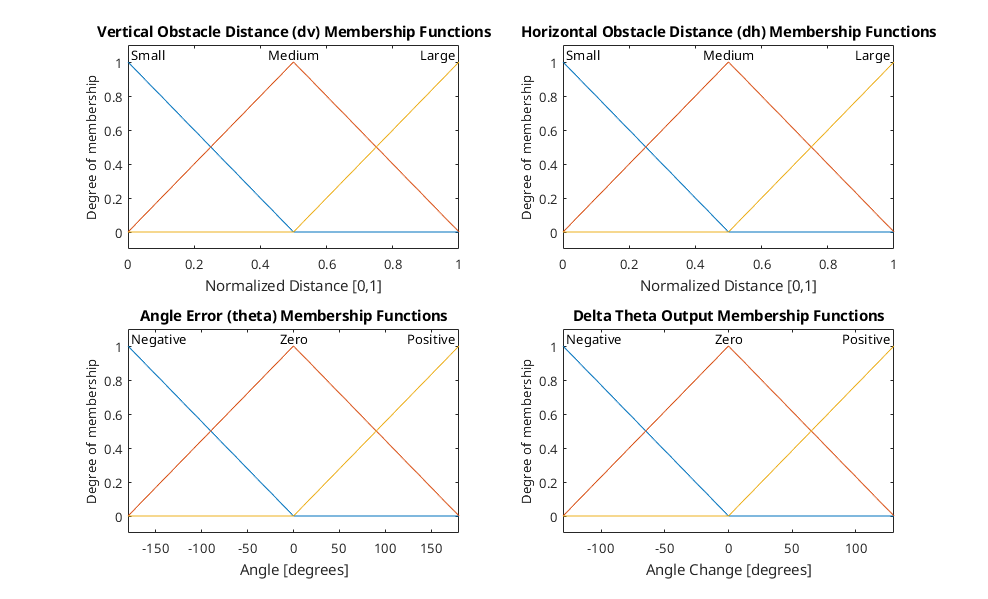
\includegraphics[width=1\textwidth]{figures/membership_functions.png}
    \caption{Συναρτήσεις συμμετοχής για τις αποστάσεις του αυτοκινήτου από τα εμπόδια}
    \label{fig:membership_functions}
\end{figure}
Οι τροχιές που προκύπτουν για τις 3 αρχικές γωνίες είναι οι εξής:
\begin{figure}[H]
    \centering
    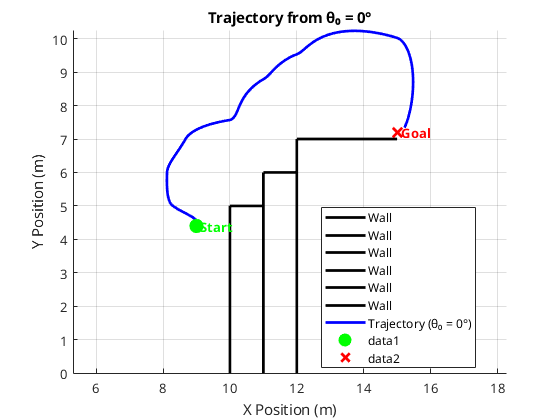
\includegraphics[width=0.8\textwidth]{figures/trajectory_1.png}
    \caption{Τροχιά για θ₀ = 0°}
    \label{fig:trajectory_1}
\end{figure}
\begin{figure}[H]
    \centering
    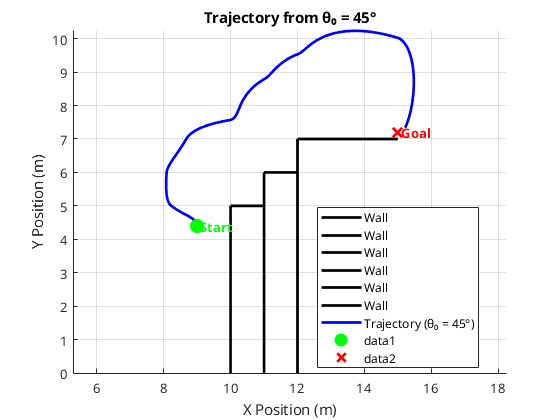
\includegraphics[width=0.8\textwidth]{figures/trajectory_2.png}
    \caption{Τροχιά για θ₀ = 45°}
    \label{fig:trajectory_2}
\end{figure}
\begin{figure}[H]
    \centering
    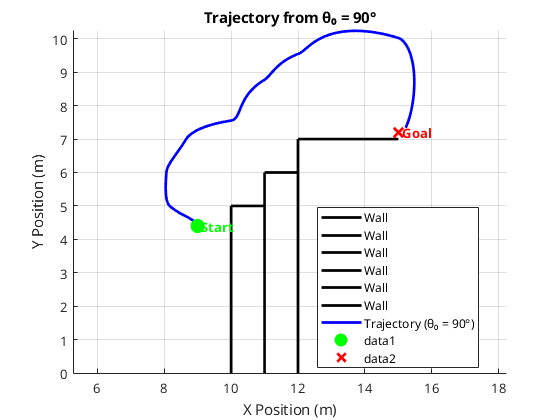
\includegraphics[width=0.8\textwidth]{figures/trajectory_3.png}
    \caption{Τροχιά για θ₀ = 90°}
    \label{fig:trajectory_3}
\end{figure}

\section{Τροποποιήσεις συναρτήσεων συμμετοχής}
Η κανονικοποίηση που κάναμε προηγουμένως προκειμένου η είσοδος να βρίσκεται εντός του πεδίου ορισμού των συναρτήσεων συμμετοχής δεν είναι πλέον απαραίτητη. Έτσι, έπειτα από την αφαίρεση του αντίστοιχου κώδικα, πρόκειται να μεταβάλλουμε τις συναρτήσεις συμμετοχής ούτως ώστε το αμάξι να μεταβαίνει πολύ πιο γρήγορα και ομαλά στην τελική του θέση. Αυτό προϋποθέτει ότι κάθε τιμή που μπορεί να πάρει το dh και το dv χαρακτηρίζεται ικανά ως μεγάλη, μεσαία ή μικρή. 

Παρατηρώντας ότι ως έχει το αμάξι αποφεύγει πολύ τους τοίχους οδηγώντας το να διαγράψει μια ιδιαίτερα περιφερειακή πορεία, δίνουμε την εντολή να στρίψει μόνο όταν η απόσταση είναι πολύ μικρή. Στην προκειμένη περίπτωση έχουμε επιλέξει την τιμή 0.3 για το δεξί τέλος της τριγωνικής συνάρτησης συμμετοχής, που αναφέρεται στην ιδιότητα μεγάλο, με το κέντρο να παραμένει ίδιο στο 0. 

Για να επιτρέψουμε στο αμάξι να λάβει μεγαλύτερες αποστάσεις dv και dh μετατρέπουμε τις dv και dh συναρτήσεις συμμετοχής σε τραπεζοειδείς, οι οποίες είναι ίδιες μέχρι το σημείο 1 και έπειτα απλά παραμένουν στο 1 μέχρι ένα άνω όριο που θέτουμε (στην συγκεκριμένη περίπτωση 20μ).

Τα αποτελέσματα των παραπάνω αλλαγών φαίνονται παρακάτω:
\begin{figure}[H]
    \centering
    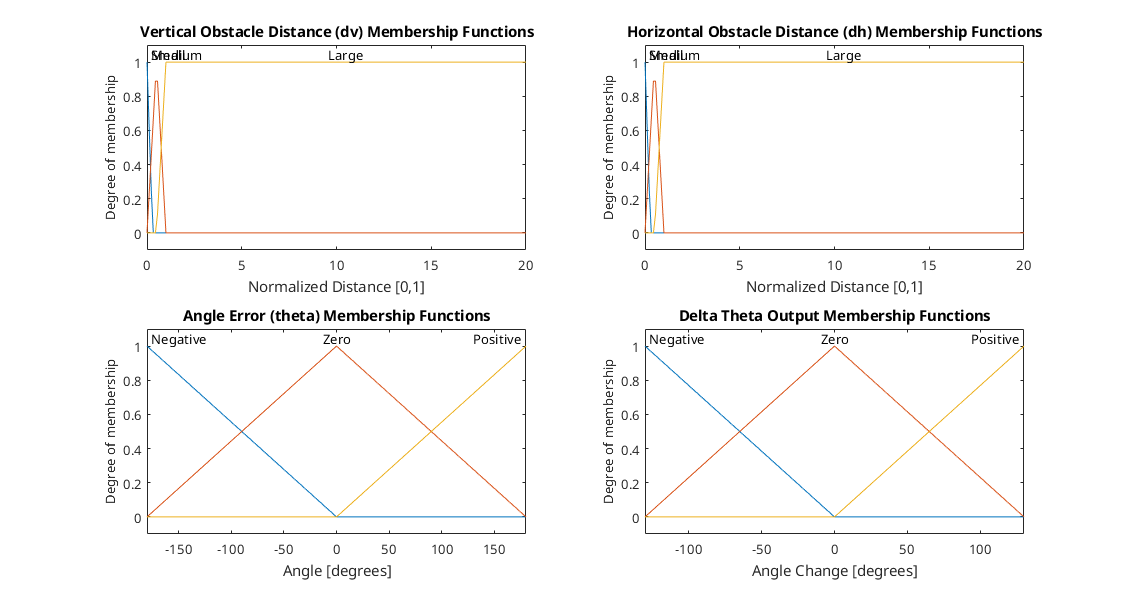
\includegraphics[width=1\textwidth]{figures/membership_functions_opt.png}
    \caption{Συναρτήσεις συμμετοχής για τις αποστάσεις του αυτοκινήτου από τα εμπόδια (Optimized MFs)}
    \label{fig:membership_functions_opt}
\end{figure}
\begin{figure}[H]
    \centering
    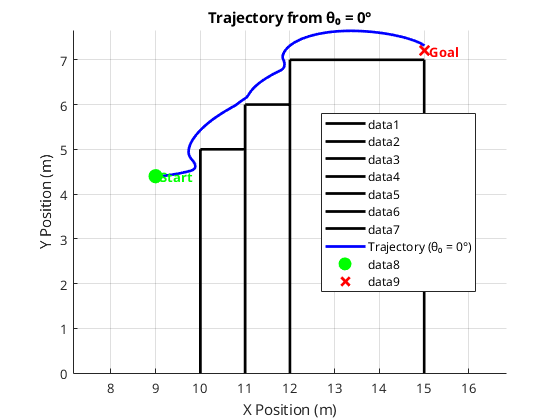
\includegraphics[width=0.8\textwidth]{figures/trajectory_opt_1.png}
    \caption{Τροχιά για θ₀ = 0° (Optimized MFs)}
    \label{fig:trajectory_opt_1}
\end{figure}
\begin{figure}[H]
    \centering
    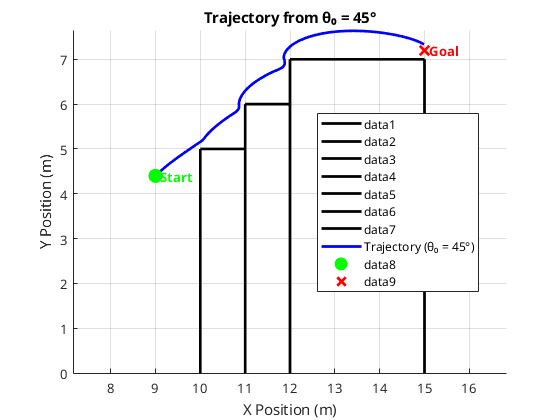
\includegraphics[width=0.8\textwidth]{figures/trajectory_opt_2.png}
    \caption{Τροχιά για θ₀ = 45° (Optimized MFs)}
    \label{fig:trajectory_opt_2}
\end{figure}
\begin{figure}[H]
    \centering
    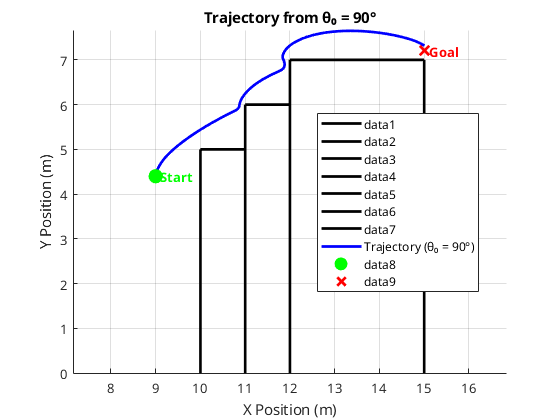
\includegraphics[width=0.8\textwidth]{figures/trajectory_opt_3.png}
    \caption{Τροχιά για θ₀ = 90° (Optimized MFs)}
    \label{fig:trajectory_opt_3}
\end{figure}

\section{Σχολιασμός αποτελεσμάτων}
Η διαμόρφωση σωστού rule base είναι κομβικής σημασίας όμως χωρίς την παροχή expert knowledge το σύστημα δεν μπορεί να ανταπεξέλθει ικανά στις προκλήσεις ενός απαιτητικού προβλήματος όπως autonomous driving.

\end{document}